\section{Barrow: Geometric Proportions and Tangents (1670)}

Isaac Barrow, the teacher of Newton, described what we now call calculus entirely through **geometric constructions**. He avoided algebra and worked with labeled curves and figures.

Let a curve \( AB \) be drawn, with perpendiculars (ordinates) erected from a baseline. Let another curve \( AP \) be constructed such that:

\begin{quote}
\textit{“The ordinate of \( AP \) at any point is proportional to the sum of the ordinates of the curve \( AB \) up to that point.”}
\end{quote}

Then, Barrow would assert:

\begin{quote}
\textit{“The tangent to the curve \( AP \) at a point is proportional to the height of the corresponding ordinate of the original curve \( AB \).”}
\end{quote}

Barrow’s geometric proof of this property was entirely visual, using proportions between small triangles drawn tangent to the area-accumulating curve and the original curve.

No functions, no coordinates—just proportions, ratios, and curves drawn carefully on a diagrammatic plane.

\vspace{1em}

\begin{center}
\textit{Cavalieri dissected shapes by indivisibles. Wallis summed their powers. Barrow reassembled them with tangents.}
\end{center}


\begin{figure}[H]
    \centering
    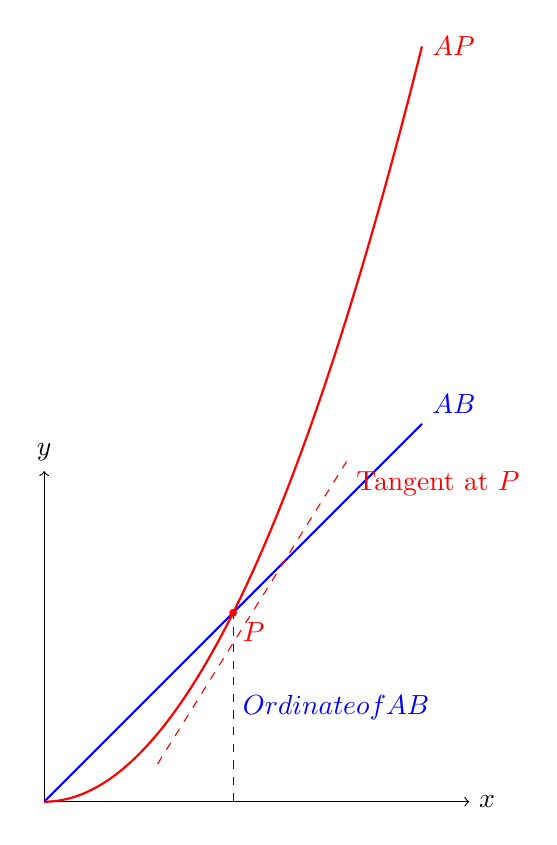
\begin{tikzpicture}[scale=1.2]
      % Axes
      \draw[->] (0,0) -- (4.5,0) node[right] {$x$};
      \draw[->] (0,0) -- (0,3.5) node[above] {$y$};
    
      % Curve AB: the "original" curve (e.g., y = x)
      \draw[thick, domain=0:4, samples=100, smooth, variable=\x, blue] 
        plot ({\x}, {\x}) node[above right] {$AB$};
    
      % Curve AP: the "area" curve (e.g., y = x^2/2)
      \draw[thick, domain=0:4, samples=100, smooth, variable=\x, red] 
        plot ({\x}, {0.5*\x*\x}) node[right] {$AP$};
    
      % Mark a point P on AP
      \filldraw[red] (2,2) circle (1pt) node[below right] {$P$};
    
      % Tangent line at P to AP
      \draw[dashed, red] (1.2,0.4) -- (3.2,3.6) node[below right] {Tangent at $P$};
    
      % Vertical ordinate on AB at x = 2
      \draw[dashed, blue] (2,0) -- (2,2) node[midway, right] {$\text{Ordinate of } AB$};
    \end{tikzpicture}
    \caption{Barrow’s Area–Tangent Construction: The height of curve $AB$ determines the slope of the tangent to the curve $AP$, whose height represents the area under $AB$.}
\end{figure}

